\chapter{LaTeX Hints}
\label{chap:latexhints}


\newenvironment{twocoldemo}[1][]{%
  \par\noindent
  \begin{minipage}[t]{.48\linewidth}\raggedright
  \textbf{Code}\par\smallskip
}{%
  \end{minipage}\hfill
  \begin{minipage}[t]{.48\linewidth}\raggedright
  \textbf{Output}\par\smallskip
  \end{minipage}\par
}



This appendix shows small, copy-pasteable examples that compile with this thesis class out of the box. It avoids any template-specific commands from other classes.

\section{Paragraphs and inline emphasis}
Write one sentence per source line (helps with version control). A blank line starts a new paragraph.

You can write \emph{emphasized (italics)} and \textbf{bold} text. Use \verb|\url{...}| for clickable links, e.g.\ \url{https://ctan.org}.

\section{Math and equations}
Inline math: $f(x)=x^2+1$. Numbered display equations use \texttt{amsmath}:
\begin{align}
  \label{eq:sample}
  \int_0^1 x^2\,dx = \frac{1}{3}.
\end{align}
We can reference \cref{eq:sample} thanks to \texttt{cleveref}.

\section{Figures and subfigures}
A normal figure:
\begin{figure}[h]
  \centering
  
\includegraphics[width=.7\linewidth]{b_chapters/chapter1/assets/RNU_large_logo.png}
  \caption{Example figure.}
  \label{fig:example}
\end{figure}

Two images side-by-side via \texttt{subcaption}:
\begin{figure}[h]
  \centering
  \begin{subfigure}{.47\linewidth}
    \centering
    
\includegraphics[width=.9\linewidth]{b_chapters/chapter1/assets/RNU_large_logo.png}
    \caption{Left}
    \label{fig:left}
  \end{subfigure}\hfill
  \begin{subfigure}{.47\linewidth}
    \centering
    
\includegraphics[width=.9\linewidth]{b_chapters/chapter1/assets/RNU_large_logo.png}
    \caption{Right}
    \label{fig:right}
  \end{subfigure}
  \caption{Two subfigures.}
  \label{fig:two-subfigs}
\end{figure}

We can reference \cref{fig:example,fig:two-subfigs,fig:left}.

\section{Tables}
A compact table with \texttt{booktabs}:
\begin{table}[h]
  \caption{Compact example table}
  \label{tab:compact}
  \centering
  \begin{tabular}{lrr}
    \toprule
    Factor & Mean & SD\\
    \midrule
    Pay           & 2.0 & 0.5\\
    Recognition   & 4.0 & 0.7\\
    Growth        & 5.0 & 0.6\\
    \bottomrule
  \end{tabular}
\end{table}

A long table across multiple pages (\texttt{longtable}):
\begin{longtable}{llr}
\caption{Long table example}\label{tab:long}\\
\toprule
\textbf{Item} & \textbf{Group} & \textbf{Value}\\
\midrule
\endfirsthead
\toprule
\textbf{Item} & \textbf{Group} & \textbf{Value}\\
\midrule
\endhead
\bottomrule
\endfoot
A & Alpha & 1\\
B & Alpha & 2\\
C & Beta  & 3\\
A & Alpha & 1\\
B & Alpha & 2\\
C & Beta  & 3\\
A & Alpha & 1\\
B & Alpha & 2\\
C & Beta  & 3\\
A & Alpha & 1\\
B & Alpha & 2\\
C & Beta  & 3\\
A & Alpha & 1\\
B & Alpha & 2\\
C & Beta  & 3\\
A & Alpha & 1\\
B & Alpha & 2\\
C & Beta  & 3\\
A & Alpha & 1\\
B & Alpha & 2\\
C & Beta  & 3\\
A & Alpha & 1\\
B & Alpha & 2\\
C & Beta  & 3\\
A & Alpha & 1\\
B & Alpha & 2\\
C & Beta  & 3\\
A & Alpha & 1\\
B & Alpha & 2\\
C & Beta  & 3\\
A & Alpha & 1\\
B & Alpha & 2\\
C & Beta  & 3\\
\end{longtable}

A landscape figure page (\texttt{pdflscape}):
\begin{landscape}
\begin{figure}[h]
  \centering
  
\includegraphics[width=.9\linewidth]{b_chapters/chapter1/assets/RNU_large_logo.png}
  \caption{Landscape example.}
\end{figure}
\end{landscape}

\section{Algorithms and code listings}
Pseudocode with \texttt{algorithm}+\texttt{algpseudocode}:
\begin{algorithm}[h]
\caption{Greedy selection (example)}
\begin{algorithmic}[1]
  \State Initialize $S \gets \emptyset$
  \While{feasible choice exists}
    \State choose best feasible item $x$
    \State $S \gets S \cup \{x\}$
  \EndWhile
  \State \Return $S$
\end{algorithmic}
\label{alg:greedy-app}
\end{algorithm}

Code with \texttt{listings}:
% \begin{lstlisting}[language=Python,caption={Bubble sort},label={lst:bubble-app}]
% def bubble(a):
%     n = len(a)
%     for i in range(n-1):
%         for j in range(n-1-i):
%             if a[j] > a[j+1]:
%                 a[j], a[j+1] = a[j+1], a[j]
% \end{lstlisting}
{\captionsetup{type=lstlisting}
\begin{lstlisting}[language=Python,caption={Bubble sort},label={lst:bubble-app}]
def bubble(a):
    n = len(a)
    for i in range(n-1):
        for j in range(n-1-i):
            if a[j] > a[j+1]:
                a[j], a[j+1] = a[j+1], a[j]
\end{lstlisting}
}



We can reference \cref{alg:greedy-app,lst:bubble-app}.

% \section{TikZ and (optional) pgfplots}
% A tiny TikZ graphic:
% \begin{figure}[h]
%   \centering
%   \begin{tikzpicture}
%     \draw (0,0) rectangle (2,1);
%     \foreach \x in {0.25,0.5,...,1.75} \draw (\x,0.5) circle (1pt);
%   \end{tikzpicture}
%   \caption{Simple TikZ demo.}
% \end{figure}

\par\noindent
\section{TikZ: Trie data structure diagram}

TikZ is a powerwfull diagraming, graphing engine allowing you to script creation of the
diagrams. Refer to \url{https://tikz.dev/} for online documentation and examples.

\begin{figure}[h]
  \centering
  \tikz [>={To[sep]}, rotate=90, xscale=-1,
         mark/.style={fill=black!50}, mark/.default=]
    \graph [trie, simple,
            nodes={circle,draw},
            edges={nodes={
                inner sep=1pt, anchor=mid,
                fill=yellow!20}}, % yellowish background
            put node text on incoming edges]
      {
        root[mark] -> {
          a -> n -> {
            g [mark],
            f -> a -> n -> g [mark]
          },
          f -> a -> n -> g [mark],
          g[mark],
          n -> {
            g[mark],
            f -> a -> n -> g[mark]
          }
        },
        { [edges=red] % highlight one path
          root -> f -> a -> n
        }
      };
  \caption{Trie data structure demonstrating graph-based TikZ syntax with highlighted path.}
  \label{fig:tikz-trie-demo}
\end{figure}


If \texttt{pgfplots} is installed (we auto-load it if present), a quick plot:
\IfFileExists{pgfplots.sty}{%
\begin{figure}[h]
  \centering
  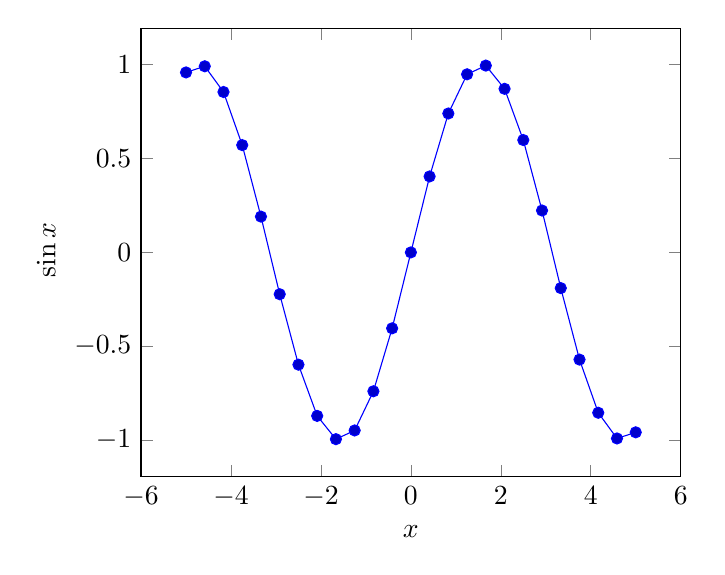
\begin{tikzpicture}
    \begin{axis}[xlabel=$x$,ylabel={$\,\sin x$}]
      \addplot {sin(deg(x))};
    \end{axis}
  \end{tikzpicture}
  \caption{Sine plot with pgfplots.}
\end{figure}
}{\noindent\emph{(pgfplots not installed — skipping plot.)}}

\section{Cross-references}
Use \verb|\label{...}| and \verb|\cref{...}| for equations, figures, tables, algorithms, and listings to get correct names and numbers automatically.

\section{Bibliography citation}
Cite like \cite{porter2008} and list all sources in the “Literature” section (managed by \texttt{biblatex} with the IEEE style in this project).
